%===============================================================================
% APPENDIX: MODEL ARCHITECTURE
%===============================================================================
\section{Model Architecture}
\label{app:architecture}
%===============================================================================

This section provides a comprehensive overview of the core architectural components of our model, detailing both the novel GraphPathway Encoder and the deep causal graph learning framework.

%-------------------------------------------------------------------------------
% Subsection: GraphPathway Encoder Architecture
%-------------------------------------------------------------------------------
\subsection{Overview of RAPTORGraph framework}
\label{app:architecture:overview}
%-------------------------------------------------------------------------------

The architecture of the \gls{raptorgraph} framework, illustrated in \cref{fig:app:architecture:overview}, is designed as an end-to-end system for learning causal relationships from interventional single-cell data.
The framework is composed of three primary modules: a preconditioned encoder for sparse representation learning, a DAG discovery layer for identifying causal structure, and a decoder for reconstructing cellular states.

The input to the model is the high-dimensional gene expression data.
The first layer of the encoder is our novel preconditioned GraphPathway Encoder, which addresses the Intervention Spillover Problem.
By leveraging prior biological knowledge, it enforces a sparse mapping from the thousands of observed genes ($\sR^{\observeddim}$) to a lower-dimensional set of learned meta-pathways ($\sR^{\latentdim}$).
This ensures that a single-gene intervention activates only a sparse, well-defined set of learned meta-pathways in the latent space, fulfilling the requirements for valid downstream causal inference.

The resulting latent representations, $\latentvars$, are then passed to the DAGMA-based DAG discovery module.
This layer operates directly on the latent variables to learn the causal relationships *between* the learned meta-pathways.
Its primary output is a directed acyclic graph ($\graph$), represented by its adjacency matrix, which models the flow of biological influence among the learned meta-pathways.

Finally, the decoder network reconstructs the original gene expression profile from the latent representation.
This ensures that the latent variables, in addition to being causally structured, also retain sufficient information to accurately capture the full cellular state.
The model is trained end-to-end by optimizing a composite loss function that balances these different objectives, as detailed in the figure caption.

\begin{figure}[H]
    \centering
    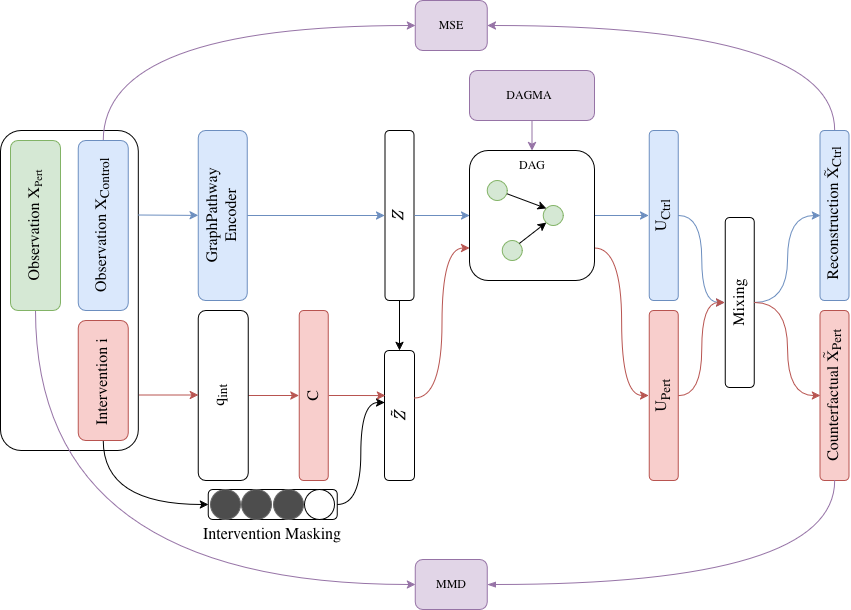
\includegraphics[width=.8\textwidth]{gfx/full_framework_modified.png}
    \caption{
        Detailed schematic of the \gls{raptorgraph} framework.
        The preconditioned GraphPathway Encoder enforces a sparse mapping from the high-dimensional gene expression space ($\sR^{\observeddim}$) to the learned meta-pathways ($\sR^{\latentdim}$).
        The DAGMA-based DAG operates on the latent representations to learn a directed acyclic graph ($\graph$) representing the causal relationships between the learned meta-pathways.
        The model is trained end-to-end using a composite loss function comprised of several terms: a reconstruction loss (\gls{mse}), a distributional loss (\gls{mmd}) on interventional predictions, a KL Divergence on the \gls{vae} latent variables, and an acyclicity constraint from the DAGMA layer.
    }
    \label{fig:app:architecture:overview}
\end{figure}

%-------------------------------------------------------------------------------
% Subsection: GraphPathway Encoder Architecture
%-------------------------------------------------------------------------------
% [ADDITION: Addressing Reviewer yvAn] Reinforcing the end-to-end/joint optimization nature 
% of the GraphPathway encoder and DAGMA module.
\revised{The entire framework is trained end-to-end. During optimization, gradients from the \glsentryshort{dagma} loss $\dagmaloss$ backpropagate through the GraphPathway encoder, ensuring that the latent representation is regularized to expose the underlying causal structure.}

%-------------------------------------------------------------------------------
\subsection{Joint Discovery via Causal Transform Layer}
\label{app:arch:causal_transform}
%-------------------------------------------------------------------------------

A common misunderstanding in causal representation learning is the perceived decoupling between representation learning (\glsentryshort{vae}) and causal structure learning (\glsentryshort{dag} discovery). In \glsentryshort{raptorgraph}, these components are architecturally integrated through a \textbf{Causal Transform} layer.

\paragraph{1. The Causal Layer in the Forward Pass}
The \glsentryshort{dag} module is not a post-hoc analysis tool; it is a differentiable layer situated between the encoder and the decoder. In the forward pass, the exogenous noise $\exonoise$ (output of the GraphPathway encoder) is transformed into endogenous pathway activities $\latentcausalvars$ by solving the structural equation:
\begin{equation}
    \latentcausalvars = \latentcausalvars \graphmatrix^T + \exonoise \implies \latentcausalvars = \exonoise(\identitymatrix - \graphmatrix)^{-T}
\end{equation}
where $\graphmatrix$ is the learnable adjacency matrix. This $\latentcausalvars$ is then passed to the decoder to produce the reconstruction $\predictedvariable$.

\paragraph{2. Joint Optimization by Reconstruction}
Because the \glsentryshort{dag} layer is part of the autoencoder's forward pass, the reconstruction loss $\mseloss = \|\variables - \predictedvariable\|^2$ backpropagates gradients through the decoder, the \glsentryshort{dag} layer ($\graphmatrix$), and the encoder. This ensures that the latent space and the causal graph are \textbf{jointly optimized} to satisfy the data-fit objective. 

%-------------------------------------------------------------------------------
\subsection{The Necessity of Hard Architectural Constraints vs. Soft Alignment}
\label{app:arch:hard_vs_soft}
%-------------------------------------------------------------------------------

We formally justify the use of hard architectural constraints (the GraphPathway encoder) over soft alignment mechanisms (e.g., concept bottleneck supervision).

\paragraph{1. Preventing Intervention Spillover}
Dense encoders (MLPs) suffer from intervention spillover, where a sparse perturbation in gene space propagates into a dense signal in latent space. While soft losses can encourage alignment, they do not provide the \textbf{guaranteed isolation} required for identifiable causal discovery. The hard GraphPathway constraint ensures that the interventional entry point is architecturally limited to a unique node ($\nabla_{do(x_i)} z_j = 0$ for $i \neq j$), eliminating the "winner-take-all" misattribution common in soft-aligned models.

\paragraph{2. Preserving Biological Interpretability for GI Scoring}
The identification of complex Genetic Interactions (e.g., Synergy, Redundancy) requires a strict 1-1 mapping between perturbation targets and causal factors. Soft alignment often leads to "leaky" representations where a single biological program is smeared across multiple latent variables. Our results demonstrate that the hard structural constraint is essential for maintaining the fidelity required to score these non-additive interactions accurately.

\subsection{GraphPathway Encoder Architecture}
\label{app:graphpathway}
%-------------------------------------------------------------------------------

The GraphPathway Encoder is a custom neural network layer designed to solve the Intervention Spillover Problem through a principled architectural design.
It combines a preconditioned weight matrix to deconfound known perturbation effects with a multi-subgraph structure to capture complex, non-linear gene interactions.

%-------------------------------------------------------------------------------
% Subsubsection: Deconfounding through Preconditioning
%-------------------------------------------------------------------------------
\subsubsection{Deconfounding through Preconditioning}
\label{app:graphpathway:preconditioning}
%-------------------------------------------------------------------------------

The foundational component of the encoder is its preconditioned weight matrix, which enforces the single-node intervention assumption required for causal identifiability.
As described in \cref{subsec:methods:graphpathway}, the layer's primary weight matrix $\weightmatrix$ is structured as a block matrix with a strictly diagonal top-left block.
This structure guarantees that each known perturbed gene has a direct, isolated influence on exactly one latent pathway, while the zero-block explicitly prevents its effect from spilling over into other pathways.
This design transforms the encoder into a deterministic modulator for known interventions, allowing the intervention mask $\maskvector$ to be fixed by the architecture rather than being a learned (and potentially dense) variable.
\revised{By explicitly blocking the spillover of the intervention effect into other pathways via the zero-block,} this design transforms the encoder into a deterministic modulator for known interventions, allowing the intervention mask $\maskvector$ to be fixed by the architecture rather than being a learned (and potentially \revised{confounded}) variable.

%-------------------------------------------------------------------------------
% Subsubsection: Modeling Non-Linear Interactions with Subgraphs
%-------------------------------------------------------------------------------
\subsubsection{Modeling Non-Linear Interactions with Subgraphs}
\label{app:graphpathway:subgraphs}
%-------------------------------------------------------------------------------

To move beyond a purely linear model and capture the complex, non-linear dynamics of biological processes, the architecture learns $\numgraphs$ distinct representations for each pathway.
This is achieved by first applying a masked linear layer that maps the input genes $\variables$ to an intermediate representation.
This layer's weight matrix is derived by repeating the base preconditioned mask $\numgraphs$ times, creating $\numgraphs$ parallel, similarly conditioned subgraphs that are initialized differently to learn diverse feature mappings.
The initial activation vector, $\pathwayactivation^{(g)}$, for each subgraph $g$ is computed as:
\begin{equation}
    \pathwayactivation^{(g)} = \activationfunc(\weightmatrix^{(1, g)}\variables + \vect{b}^{(1,g)}) \quad \text{for } g=1, \dots, \numgraphs
\end{equation}
where each layer-specific weight matrix $\weightmatrix^{(1, g)}$ has the same block-diagonal structure.

An intermediate \emph{Interaction Block} then processes these subgraph activations to model higher-order dependencies.
This block applies a series of pathway-specific linear transformations and non-linear activations to the set of $\numgraphs$ activations within each pathway, enabling the model to learn complex interactions between the different feature mappings before the final aggregation step.

Finally, the processed subgraph activations are aggregated into the final pathway representations using a grouped 1D convolution.
This operation has a kernel size of $\numgraphs$ and is configured with $\latentdim$ groups, making it equivalent to applying a separate, pathway-specific linear layer to the set of $\numgraphs$ subgraph activations for each pathway.
This learns an optimal linear combination of the non-linear subgraph features to produce the final parameters for the latent distributions, $\vect{\mu}_{\latentvars}$ and $\vect{\sigma}_{\latentvars}$.

%-------------------------------------------------------------------------------
% Subsubsection: Implementation Details of GraphPathway
%-------------------------------------------------------------------------------
\subsubsection{Implementation Details of GraphPathway}
\label{app:graphpathway:implementation}
%-------------------------------------------------------------------------------

The specific implementation used in our model is the `InteractingGraphPathwayLayer`.
This layer encapsulates the preconditioning, multi-subgraph mapping, and interaction blocks into a single module.
To model complex, non-linear biological processes, each pathway learns its own unique set of interaction weights within the interaction block.
This design provides greater expressive power, as it allows the model to capture distinct interaction dynamics for each biological process.
When configured for a variational autoencoder, the output channel dimension of the final grouped convolution is doubled, allowing the layer to directly produce both the mean $\vect{\mu}_{\latentvars}$ and variance $\vect{\sigma}_{\latentvars}$ for each latent pathway.

%-------------------------------------------------------------------------------
% Subsection: Deep Causal Graph Learning with DAGMA
%-------------------------------------------------------------------------------
\subsection{Deep Causal Graph Learning with DAGMA}
\label{app:dagma}
%-------------------------------------------------------------------------------

This subsection details the DAGMA framework for causal discovery, the rationale for its adaptation within our deep learning model, and the key implementation principles required for stable and effective graph learning in a \gls{vae} context.

%-------------------------------------------------------------------------------
% Subsubsection: Theoretical Background: From NOTEARS to DAGMA
%-------------------------------------------------------------------------------
\subsubsection{Theoretical Background: From NOTEARS to DAGMA}
\label{app:dagma:background}
%-------------------------------------------------------------------------------

A fundamental challenge in causal discovery is the combinatorial nature of learning a \gls{dag}, as the number of possible graphs grows super-exponentially with the number of variables.
A breakthrough was achieved by NOTEARS~\citep{zheng2018dags}, which reformulated this discrete problem into a continuous optimization problem amenable to gradient-based methods.
The core innovation was a differentiable function, $h(\graphmatrix)$, whose value is zero if and only if the weighted adjacency matrix $\graphmatrix$ represents a \gls{dag}.
The original NOTEARS constraint is based on the matrix exponential:
\begin{equation}
    h(\graphmatrix) = \tr(e^{\graphmatrix \circ \graphmatrix}) - \latentdim = 0
    \label{eq:app:notears_constraint}
\end{equation}
where $\tr(\cdot)$ is the trace of the matrix and $\graphmatrix \circ \graphmatrix$ is the element-wise (Hadamard) product.
This function cleverly sums all cycles of all possible lengths in the graph; it equals zero only if no cycles exist.

DAGMA~\citep{bello2022dagma} builds upon this continuous optimization framework but introduces a new, log-determinant-based acyclicity characterization that often leads to faster and more stable convergence.
The DAGMA acyclicity constraint is:
\begin{equation}
    h_s(\graphmatrix) = -\log\det(s\identitymatrix - \graphmatrix \circ \graphmatrix) + \latentdim\log s = 0
    \label{eq:app:dagma_constraint}
\end{equation}
where $s>0$ is a scaling scalar.
This function is based on the principle that a matrix corresponds to a \gls{dag} if and only if all eigenvalues of its squared adjacency matrix are zero.
The log-determinant acts as a barrier, approaching infinity as the graph's structure approaches a cycle, while being minimized at zero exclusively for \glspl{dag}.

%-------------------------------------------------------------------------------
% Subsubsection: The DAGMA Optimization Framework
%-------------------------------------------------------------------------------
\subsubsection{The DAGMA Optimization Framework}
\label{app:dagma:optimization}
%-------------------------------------------------------------------------------

The full optimization problem is to minimize a score function that measures how well the graph fits the data, subject to the acyclicity constraint.
For a linear model with latent variables $\latentvars$, the score function $\scorefunc(\graphmatrix)$ is typically the mean squared error of reconstruction:
\begin{equation}
    \scorefunc(\graphmatrix) = \frac{1}{2n} \lVert \latentvars - \latentvars\graphmatrix \rVert_F^2
    \label{eq:app:dagma_score}
\end{equation}
The original DAGMA paper proposes a path-following approach that solves a sequence of unconstrained optimization problems:
\begin{equation}
    \min_{\graphmatrix} (\mu \cdot \scorefunc(\graphmatrix) + h_s(\graphmatrix))
\end{equation}
where $\mu$ is a hyperparameter that is gradually decreased towards zero during training.
As $\mu \to 0$, the penalty on violating acyclicity becomes infinitely strong, forcing the final solution for $\graphmatrix$ to be a \gls{dag}.

%-------------------------------------------------------------------------------
% Subsubsection: Rationale for a Modified DAGMA in a Causal Representation Learning
%-------------------------------------------------------------------------------
\subsubsection{Rationale for a Modified DAGMA in a Causal Representation Learning}
\label{app:dagma:rationale}
%-------------------------------------------------------------------------------

Integrating DAGMA into a \gls{vae} for interventional \gls{crl} requires careful design to ensure the model learns a meaningful causal graph.
Our implementation is guided by two core principles.

\paragraph{Principle 1: Learning the Invariant Graph from Observational Data.}
A foundational assumption is that the causal graph $\graphmatrix$ represents an invariant, underlying mechanism of the system.
Therefore, the DAGMA loss, which encourages the learning of this structure, must be computed exclusively on the latent representations of observational data ($\zobs$).
This teaches the model the fundamental causal rules from the system's natural dynamics.
The interventional data and their latent representations ($\zint$) are used to compute a separate discrepancy loss (e.g., \gls{mmd}).
This second loss teaches the model the consequences of breaking the causal rules, evaluating how well the learned graph functions as a simulator for interventions.
Applying the graph loss to interventional latents would create a conflicting objective, as an intervention by definition breaks the natural mechanism the graph is supposed to represent.

\paragraph{Principle 2: Isolating Gradient Flow via Input Detachment.}
The most critical design principle for stability is isolating the gradient flow between the \gls{vae}'s encoder and the DAGMA layer.
This is achieved by detaching the latent variable tensor ($\zobs$) before it is used in the score calculation ($\scorefunc(\graphmatrix, \zobs\text{.detach()})$).
This design choice has two key benefits.
First, it mimics the original DAGMA algorithm, which operates on a fixed dataset.
Second, and more importantly, it creates a separation of concerns: the encoder learns to produce a rich representation, and the DAGMA layer learns the graph of that representation.
Without detaching, gradients from the DAGMA score would flow back to the encoder, encouraging it to learn a trivial, simplistic latent space that is easy to fit, thereby destroying the quality of the representation.

%-------------------------------------------------------------------------------
% Subsubsection: Implementation Detail of DAGMA
%-------------------------------------------------------------------------------
\subsubsection{Implementation Detail of DAGMA}
\label{app:dagma:stability}
%-------------------------------------------------------------------------------

Several practical considerations are crucial for the stable application of DAGMA in a deep learning context.

\paragraph{Weight Initialization and Invertibility.}
To ensure stability from the start of training, the weights of the adjacency matrix $\graphmatrix$ are initialized from a uniform distribution in the range $[-0.1, 0.1]$.
This provides the optimizer with small, non-zero weights as a starting point.
This initialization also makes it highly probable that the matrix $(\identitymatrix - \graphmatrix)$ is well-conditioned and invertible, which is critical for the forward pass of the linear DAGMA model.
The forward pass solves the structural equation $\latentvars = \latentvars\graphmatrix + \exonoise$ for $\latentvars$, which requires computing $\exonoise(\identitymatrix - \graphmatrix)^{-1}$.
To handle potential numerical instability, our implementation first attempts to solve the linear system directly.
If this fails due to a singular or ill-conditioned matrix, it robustly falls back to using the Moore-Penrose pseudo-inverse, guaranteeing a stable forward pass throughout training.

\paragraph{Input Normalization.}
A common failure mode is the collapse of the graph weights in $\graphmatrix$ to a trivial near-zero solution.
This is prevented by applying a normalization layer (e.g., `LayerNorm`) to the latent inputs ($\zobs$ and $\zint$) before they enter the DAGMA layer.
This ensures the score term has a consistent magnitude, providing a strong and stable gradient signal that encourages the model to learn a non-trivial graph.

\paragraph{Numerical Precision.}
The acyclicity constraint $h_s(\graphmatrix)$ is theoretically guaranteed to be non-negative.
However, due to floating-point limitations, it can sometimes become a very small negative number.
To handle this, the calculated value is clamped at zero, which respects the theoretical constraint while gracefully handling practical numerical artifacts.

